%\documentclass[english, 11pt]{article}
%\usepackage{haziq_article}
%\begin{document}
%\listoftodos[To-do list]

\section{Gibbs sampler for the I-prior Bayesian variable selection model}
\label{apx:gibbs}
\newcommand{\Xgam}{\mathbf X_{\boldsymbol\gamma}}

This section gives the conditional posteriors required for Gibbs sampling. This is required if self coding in R, such as for the $p > n$ case, which is not able to be run in WinBUGS or JAGS. The following derivation assumes that the data $\mathbf X$ and $\mathbf y$ have been standardised, so that the covariates are now measured on the same scale. As such, only a single scale parameter $\lambda$ is required. The advantage is that the derivation of the Gibbs conditional posteriors is much simpler. One can also use multiple scale parameters as has been described in this manuscript. However, this requires further work to derive the posteriors. Note that the scale parameter(s) can also be treated as fixed, having being estimated from the I-prior methodology. If so, then there is no conditional density for $\lambda$.

For the I-prior variable selection model stated in \eqref{eq:ipriorbvs}, the likelihood of the parameters $\boldsymbol\theta = (\boldsymbol\beta, \boldsymbol\gamma, \alpha, \psi, \lambda)$ given each observation $y_i$ and data for the $p$ covariates $x_{i1}, \dots, x_{ip}$ is iid Gaussian with mean $\mu_i = \alpha + \gamma_1\beta_1x_{i1} + \dots + \gamma_p\beta_px_{ip}$ and variance $\psi^{-1}$, for $i=1, \dots, n$. The joint prior distribution of the parameters is given by:
\[
	f(\boldsymbol\theta) = f(\boldsymbol\beta|\psi, \lambda)f(\gamma_1)\cdots f(\gamma_p)f(\alpha)f(\psi)f(\lambda^{-2}),
\]
where each of the priors are listed below:
\begin{align*}
	\begin{gathered}
		%\text{\underline{Priors for $\boldsymbol{\gamma}$, $\alpha$, and $\psi$}} \\
		\boldsymbol{\beta}|\psi,\lambda \sim \N(\mathbf b, \mathbf D) \\
		\gamma_j \sim \text{Bern}(p_j), \ j=1,\dots,p \\
		\alpha \sim \N(a,b^2) \\
		\psi, \lambda^{-2} \sim \Gamma(c,d) \ \rlap{\text{\small\color{gray} (shape and scale parameterization)}} \\
	\end{gathered}
\end{align*}
where $\mathbf b$ and $\mathbf D$ are the I-prior mean and covariance matrix for $\boldsymbol\beta$, i.e. $\mathbf b = \mathbf 0$ and $\mathbf D = \psi\boldsymbol\Lambda \mathbf X ^\top \mathbf X \boldsymbol\Lambda = \psi\lambda^2 \mathbf X ^\top \mathbf X$, since we only use one scale parameter $\lambda$ for each of the $\beta_j$s in the derivation here. Our typical choices for the hyperparameters are uninformative ones: $p_1=\dots=p_p=1/2$, $a=0$, $b^2=1000$, $c=d=0.001$.

\subsection[Conditional posterior for beta]{Conditional posterior for $\boldsymbol\beta$}

\begin{align*}
	f(\boldsymbol\beta|\mathbf y,\boldsymbol\gamma, \alpha, \psi, \lambda)
	&\propto \text{likelihood}\times f(\boldsymbol\beta|\psi, \lambda) \\
	&\equiv \N(\tilde{\mathbf b}, \tilde{\mathbf D})
\end{align*}
\begin{align*}
	\begin{gathered}
		\tilde{\mathbf b} = (\mathbf D^{-1} + \psi\Xgam^\top\Xgam)^{-1}(\mathbf D^{-1}\mathbf b + \psi\Xgam\mathbf y) \\
		\tilde{\mathbf D} = (\mathbf D^{-1} + \psi\Xgam^\top\Xgam)^{-1} \\
		\Xgam = [\gamma_1\mathbf X_1, \dots, \gamma_p\mathbf X_p] \\
		\mathbf X_j = (x_{1,j}, \dots, x_{n,j})^\top
	\end{gathered}
\end{align*}


\subsection{Conditional posterior for $\gamma_1,\dots,\gamma_p$}

\begin{align*}
	f(\gamma_j|\mathbf y,\boldsymbol\beta, \boldsymbol\gamma_{-j}, \alpha, \psi, \lambda)
	&\propto \text{likelihood}\times f(\boldsymbol\gamma_{-j}) \\
	&\equiv \text{Bern}(\tilde{p_j})
\end{align*}
\begin{align*}
	\begin{gathered}
		\boldsymbol\gamma_{-j} = (\gamma_1, \dots, \gamma_{j-1}, \gamma_{j+1}, \dots, \gamma_p) \\
		\tilde{p_j} = u_j/(u_j + v_j) \\
		u_j = p_j \exp \left[-\frac{\psi}{2} (\mathbf y -  \mathbf X \boldsymbol\phi^1)^\top (\mathbf y -  \mathbf X \boldsymbol\phi^1)\right] \\
		v_j = (1-p_j) \exp \left[-\frac{\psi}{2} (\mathbf y -  \mathbf X \boldsymbol\phi^0)^\top (\mathbf y -  \mathbf X \boldsymbol\phi^0)\right] \\
		\boldsymbol\phi = \boldsymbol\gamma^\top\boldsymbol\beta \\
		\boldsymbol\phi^1 = \boldsymbol\phi, \text{ with $j$-th entry replaced by } \beta_j \\
		\boldsymbol\phi^0 = \boldsymbol\phi, \text{ with $j$-th entry replaced by } 0
	\end{gathered}
\end{align*}

\subsection{Conditional posterior for $\psi$}

\begin{align*}
	f(\psi|\mathbf y,\boldsymbol\beta, \boldsymbol\gamma, \alpha, \lambda)
	&\propto \text{likelihood}\times f(\boldsymbol\beta|\psi, \lambda)f(\psi) \\
	&\propto \psi^{(n-p)/2+c-1} \exp \Bigg[-\frac{\sum_{i=1}^n(y_i-\mu_i)^2/2 + 1/d}{\psi^{-1}} \\
	& \hspace{6cm} - \frac{\lambda^2 \boldsymbol\beta^\top (\mathbf X^\top \mathbf X)^{-1}\boldsymbol\beta/2}{\psi} \Bigg]
\end{align*}
This is not in a closed nor identifiable form, so we have to do a Metropolis-Hastings step.

\subsubsection{Metropolis-Hastings step for $\psi$}

Let $g$ be the density for $\psi$ (given all the other parameter values) that we wish to sample from, where
\begin{align*}
	g(\psi)
	&:= \text{likelihood}\times f(\boldsymbol\beta|\psi, \lambda)f(\psi) \\
	&\equiv N(\boldsymbol\alpha +  \Xgam \boldsymbol\beta, \psi\mathbf I_n) \times 
	N(\mathbf 0, \psi\lambda^2 \mathbf X ^\top \mathbf X ) \times \Gamma(c,d).
\end{align*}

We choose a Normal proposal density for $\sigma^2:=1/\psi$ (the variance) given the current value $\sigma^2_t=1/\psi_t$, but only the absolute values are returned, i.e. $q(\sigma^2|\sigma^2_t) \equiv |N(\sigma^2_t, s^2)|$. More precisely, this is a folded Normal distribution. The pdf is

\[
	q(\sigma^2|\sigma^2_t) = \frac{1}{s\sqrt{2\pi}}e^{-\frac{(\sigma^2 - \sigma^2_t)^2}{2s^2}} + \frac{1}{s\sqrt{2\pi}}e^{-\frac{(\sigma^2 + \sigma^2_t)^2}{2s^2}}
\]

What's nice is that $q(\sigma^2|\sigma^2_t)$ is equivalent to $q(\sigma^2|\sigma^2_t)$ so this cancels out in the calculation of the acceptance probability. Given a current value of $\psi_t=1/\sigma^2_t$, the algorithm to sample $\psi_{t+1}$ is then

\begin{enumerate}
	\item Draw $\sigma^2_* \sim q(\sigma^2|\sigma^2_t)$.
	\item Calculate
		\[
			A = A(\sigma^2_*, \sigma^2_t) = \frac{g(\sigma^2_*)q(\sigma^2_t|\sigma^2_*)}{g(\sigma^2_t)q(\sigma^2_*|\sigma^2_t)} =  \frac{g(\sigma^2_*)}{g(\sigma^2_t)}
		\]
	\item Set
	\begin{align*}
		\psi_{t+1} =
		\begin{cases}
			1/\sigma^2_*	&\text{w.p. } A\\
			1/\sigma^2_t	&\text{w.p. } 1-A 
		\end{cases}
	\end{align*}
\end{enumerate}

\subsection{Conditional posterior for $\alpha$}

\begin{align*}
	f(\alpha|\mathbf y,\boldsymbol\beta, \boldsymbol\gamma, \psi, \lambda)
	&\propto \text{likelihood}\times f(\alpha) \\
	&\equiv N(\tilde a, \tilde b^2)
\end{align*}
\begin{align*}
	\begin{gathered}
		\tilde a =  \tilde b^2 \left(\frac{a}{b^2} + \psi \sum_{i=1}^n \big(y_i - \mathbf x_i^\gamma \cdot \boldsymbol\beta \big) \right) \\
		\tilde b^2 = \left(\frac{1}{b^2} + n\psi \right)^{-1} \\
		\mathbf x_i^\gamma = (\gamma_1 x_{i1}, \dots, \gamma_p x_{ip})^\top
	\end{gathered}
\end{align*}

\subsection{Conditional posterior for $\lambda^2$}
\vspace{-3mm}

\begin{align*}
	f(\lambda^2|\mathbf y,\boldsymbol\beta, \boldsymbol\gamma, \alpha, \psi) 
	&\propto f(\boldsymbol\beta|\sigma^2, \lambda)f(\lambda^{-2}) \\ 
	&\equiv \Gamma^{-1}(\tilde c, 1/\tilde d \, )
\end{align*}
\begin{align*}
	\begin{gathered}
		\tilde c =  n/2 -1 \\
		\tilde d = \left( \frac{\psi}{2} \boldsymbol\beta^\top (\mathbf X^\top \mathbf X)^{-1}\boldsymbol\beta + \frac{1}{d} \right)^{-1}
	\end{gathered}
\end{align*}
For samples of $\lambda$, take positive square roots of samples from $f(\lambda^2|\mathbf y,\boldsymbol\beta, \boldsymbol\gamma, \alpha, \psi)$. It may be useful to know that if $X \sim \Gamma(c,d)$, then $1/X \sim \Gamma^{-1}(c,1/d)$.

\vspace{-3mm}
\section{Description of datasets}
\vspace{-2mm}

\subsection{Air pollution and mortality dataset}
\label{apx:airpollution}
\vspace{-1mm}

\begin{table}[H]
\centering
\begin{tabular}{p{2.1cm}p{11.5cm}}
\textbf{Variable}     & \textbf{Description}                                                                                              \\
\hline
\texttt{Mortality}    & (RESPONSE VARIABLE) Total age adjusted mortality rate.                                                    \\
\texttt{Rain}         & Mean annual precipitation in inches.                                                                      \\
\texttt{JanTemp}      & Mean January temperature in degrees Fahrenheit.                                                           \\
\texttt{JulTemp}      & Mean July temperature in degrees Fahrenheit.                                                              \\
\texttt{Over65}       & Percent of 1960 Standard Metropolitan Statistical Area (SMSA) population that is 65 years of age or over. \\
\texttt{Popn}         & Population per household, 1960 SMSA.                                                                      \\
\texttt{Educ}         & Median school years completed for those over 25 in 1960 SMSA.                                             \\
\texttt{Hous}         & Percentage of sound housing units (no defects) with all facilities.                                       \\
\texttt{Dens}         & Population per square mile in urbanized area in 1960.                                                     \\
\texttt{NonW}         & Percent of 1960 urbanized area population that is non-white.                                              \\
\texttt{WhiteCol} & Percent employment in white-collar urbanized occupations in 1960.                                    \\
\texttt{Poor}         & Percent of families with income under \$3,000 in 1960 urbanized area.                                     \\
\texttt{Humid}        & Percent relative humidity, annual average at 1 p.m.                                                      \\
\texttt{HC}           & Relative population potential of hydrocarbons.                                                            \\
\texttt{NOx}          & Relative pollution potential of oxides of nitrogen.                                                      \\
\texttt{SO2}          & Relative pollution potential of sulphur dioxide.                                                         
\end{tabular}
\label{tab:airpollution}
\caption{Description of the air pollution data set for the analysis done in Section \ref{sec:airpollution}.}
\end{table}
\vspace{-5pt}

The sample correlations are given in the figure below. These show variables with correlations greater than 0.5 in magnitude. There are several correlations which are deducible, such as those relating to weather, or those relating to socioeconomic variables. There are also correlations which are quite surprising, such as the correlation between being underprivileged and the temperature in January and July. These are surely spurious.

\begin{figure}[H]
	\centering
	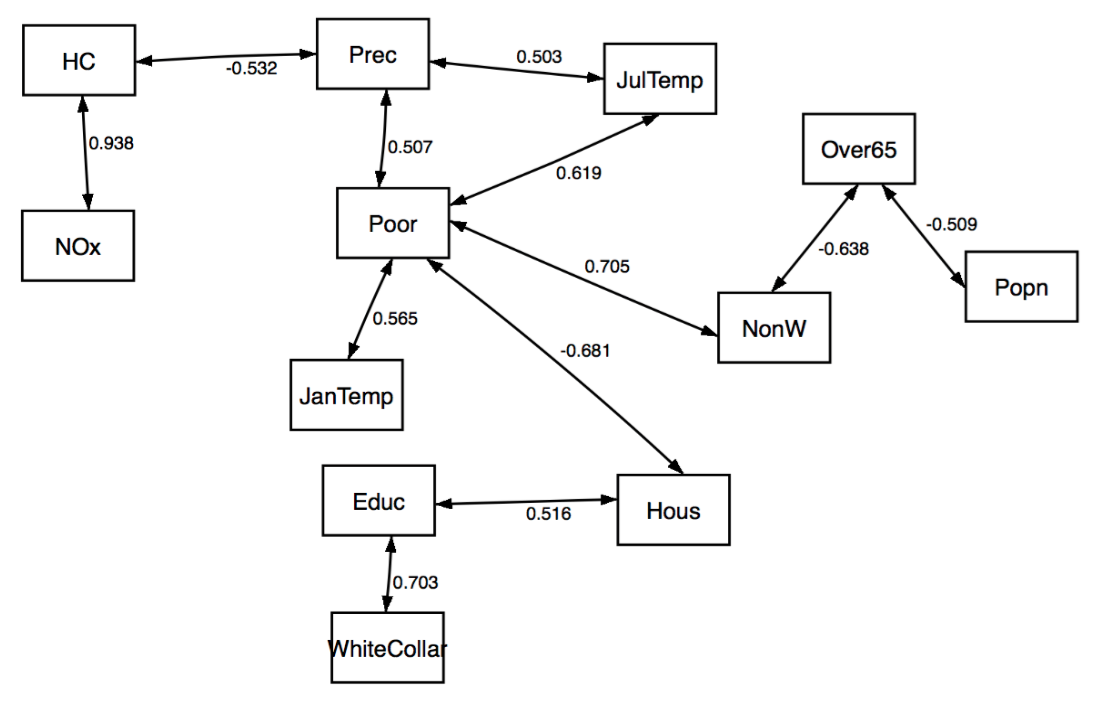
\includegraphics[height=3.5in]{figure/pollution-cor}
	\label{fig:pollution-cor}
	\caption{The sample correlations of interest in the air pollution dataset. }
\end{figure}

\subsection{Ozone dataset}
\label{apx:ozone}

\begin{table}[H]
\centering
\begin{tabular}{p{2.1cm}p{11.5cm}}
\textbf{Variable}     & \textbf{Description} \\
\texttt{Ozone}      & (RESPONSE VARIABLE) Daily maximum one-hour-average ozone reading in parts per million. \\
\texttt{Month}     & Month: $1 = \text{January}, \dots, 12 = \text{December}$ .                                      \\
\texttt{DayMonth}  & Day of month: $1,2,\dots$.                                                                 \\
\texttt{DayWeek}   & Day of week: $1 = \text{Monday}, \dots, 7 = \text{Sunday}$.                                    \\
\texttt{PresVand}  & 500 millibar pressure height (m) measured at Vandenberg AFB.                  \\
\texttt{WindLAX}   & Wind speed (mph) at Los Angeles International Airport (LAX).                  \\
\texttt{HumLAX}    & Humidity (\%) at LAX.                                                         \\
\texttt{TempSand}  & Temperature (degrees Fahrenheit) measured at Sandburg, CA.                             \\
\texttt{TempElMon} & Temperature (degrees Fahrenheit) measured at El Monte, CA.                             \\
\texttt{ibhLAX}   & Inversion base height (feet) at LAX.                                          \\
\texttt{PresGrad}  & Pressure gradient (mmHg) from LAX to Daggett, CA.                            \\
\texttt{ibtLAX}    & Inversion base temperature (degrees Fahrenheit) at LAX.                               \\
\texttt{VisLAX}    & Visibility (miles) measured at LAX.                                          
\end{tabular}
\caption{Description of the ozone data set for the analysis done in Section \ref{sec:ozone}}
\label{tab:ozone}
\end{table}

\newpage
\section{Unimodality of posterior density of I-prior model}

The hierarchical representation of the I-prior model is:

\begin{align*}
	\begin{gathered}
		\mathbf y | \boldsymbol\beta, \sigma^2 \sim \N(\mathbf X \boldsymbol\beta, \sigma^2 \mathbf I_n) \\
		\boldsymbol\beta | \lambda, \sigma^2 \sim \N \left( \mathbf 0, \frac{\lambda^2}{\sigma^2} \mathbf X^\top \mathbf X \right) \\
		(\lambda^2, \sigma^2) \sim \pi(\lambda^2) \pi(\sigma^2)
	\end{gathered}
\end{align*}

Here, the intercept parameter is not estimated. This can be done, for example, by centering all $\mathbf X$ and $\mathbf y$ variables. The log posterior is

\begin{align*}
	\log f(\boldsymbol{\beta}, \lambda^2, \sigma^2 | \mathbf y) 
	&= c + \log f(\mathbf y | \boldsymbol{\beta}, \lambda^2, \sigma^2) + \log \pi(\boldsymbol{\beta}, \lambda^2, \sigma^2) \\
	&= c + \log f(\mathbf y | \boldsymbol{\beta}, \lambda^2, \sigma^2) + \log \pi(\boldsymbol{\beta} | \lambda^2, \sigma^2) + \log \pi(\lambda^2, \sigma^2) \\
	&= c - \frac{n}{2} \log \sigma^2 - \frac{1}{2\sigma^2} \Vert \mathbf y - \mathbf X \boldsymbol{\beta} \Vert^2 - \frac{1}{2} \log \left\vert \frac{\lambda^2}{\sigma^2} \mathbf X^\top \mathbf X \right\vert \\
	& -\frac{\sigma^2}{2\lambda^2} \boldsymbol{\beta}^\top (\mathbf X^\top \mathbf X)^{-1} \boldsymbol{\beta} + \log \pi(\sigma^2) + \log \pi(\lambda^2) \\
	&= c + \log \pi(\sigma^2) + \log \pi(\lambda^2) - \frac{n-p}{2} \log \sigma^2 - \frac{1}{2\sigma^2} \Vert \mathbf y - \mathbf X \boldsymbol{\beta} \Vert^2 \\
	&  - \frac{p}{2} \log \lambda^2 -\frac{\sigma^2}{2\lambda^2} \boldsymbol{\beta}^\top (\mathbf X^\top \mathbf X)^{-1} \boldsymbol{\beta} 
\end{align*}

Change variables
\begin{align*}
	\begin{gathered}
		\boldsymbol\phi \leftrightarrow \boldsymbol{\beta}/\sigma \\
		\rho \leftrightarrow 1/\sigma
	\end{gathered}
\end{align*}

Becomes
\begin{align*}
	\log f(\boldsymbol{\beta}, \lambda^2, \sigma^2 | \mathbf y)
	&= c + \log \pi(1/\rho^2) + \log \pi(\lambda^2) + (n-p) \log \rho - \frac{1}{2} \Vert \rho\mathbf y - \mathbf X \boldsymbol{\phi} \Vert^2 \\
	&  - \frac{p}{2} \log \lambda^2 -\frac{1}{2\lambda^2\rho^4} \boldsymbol{\phi}^\top (\mathbf X^\top \mathbf X)^{-1} \boldsymbol{\phi} 
\end{align*}


%%%%%%%%%%%%%%%%%%%%%%%%%%%%%%%%%%%%%%%%%%%%%%%%%%%%%%%%%%%%%%%%%%%%%%%%
%%% REFERENCES %%%%%%%%%%%%%%%%%%%%%%%%%%%%%%%%%%%%%%%%%%%%%%%%%%%%%%%%%
%%%%%%%%%%%%%%%%%%%%%%%%%%%%%%%%%%%%%%%%%%%%%%%%%%%%%%%%%%%%%%%%%%%%%%%%
%\nocite{*}
%\bibliographystyle{apalike}
%\bibliography{haziq}
%\end{document}












